documentclass[conference]{IEEEtran}
\pagestyle{empty}

\usepackage{cite}
\usepackage{amsmath,amssymb,amsfonts}
\usepackage{algorithmic}
\usepackage{algorithm}
\usepackage{graphicx}
\graphicspath{{./}{./figures/}}
\usepackage{textcomp}
\usepackage{xcolor}
\usepackage{array}
\usepackage{booktabs}
\usepackage{url}

% ---- Placeholder figure box ----
% Usage: \screenshotbox{height}{label text}
\newcommand{\screenshotbox}[2]{%
  \fbox{\parbox[c][#1][c]{0.95\columnwidth}{\centering
    \vspace{0.5em}
    \textbf{[ PASTE SCREENSHOT HERE ]}\\[0.4em]
    \small #2
    \vspace{0.5em}
  }}%
}

\begin{document}

\title{Smart Infrastructure Intelligence System (SIIS): Multi-Model Detection, Spatial Clustering, and Priority Triage for Urban Roadways and Sanitation}

\author{
\begin{minipage}[t]{0.31\textwidth}
\centering
\textsuperscript{1}Manoj Cherukuri\\
\textit{\small Dept. of Computer Science \& Eng.,}\\
\textit{\small Vel Tech Rangarajan Dr. Sagunthala}\\
\textit{\small R\&D Institute of Sci. \& Tech.,}\\
{\small Chennai, India}\\
{\footnotesize vtu25721@veltech.edu.in}
\end{minipage}
\hfill
\begin{minipage}[t]{0.32\textwidth}
\centering
\textsuperscript{2}B. Srikar Reddy\\
\textit{\small Dept. of Computer Science \& Eng.,}\\
\textit{\small Vel Tech Rangarajan Dr. Sagunthala}\\
\textit{\small R\&D Institute of Sci. \& Tech.,}\\
{\small Chennai, India}\\
{\footnotesize vtu25754@veltech.edu.in}
\end{minipage}
\hfill
\begin{minipage}[t]{0.31\textwidth}
\centering
\textsuperscript{3}Dr. M. S. Arun Kumar\\
\textit{\small Dept. of Computer Science \& Eng.,}\\
\textit{\small Vel Tech Rangarajan Dr. Sagunthala}\\
\textit{\small R\&D Institute of Sci. \& Tech.,}\\
{\small Chennai, India}
\end{minipage}
}

\maketitle

\begin{abstract}
Municipal road and sanitation monitoring in developing cities remains largely reactive. Citizen grievance portals often accumulate unverified, duplicate complaints for identical physical defects, leaving public works departments with unranked backlogs and little actionable visual context. We present the Smart Infrastructure Intelligence System (SIIS), an end-to-end client-to-server architecture designed to convert unstructured civic reports into deduplicated, prioritized repair work orders. The vision subsystem decouples hazard analysis into three specialized YOLO models rather than a single compromised network: a YOLO26n-seg instance segmentation model for surface depressions (0.874 $\text{mAP}_{50}$ on potholes), an expanded-resolution ($768\times 768$) YOLO26s model for asphalt fractures (0.907 $\text{mAP}_{50}$), and a multi-class YOLO26s detector targeting municipal waste infrastructure defects (0.742 $\text{mAP}_{50}$ across broken containers, overflowing waste, and scattered street litter). To curb ticket inflation, reports within a 50-meter radius sharing defect classification and bounding-box geometry merge automatically into unified geospatial issue records while retaining photos as supporting evidence. A rule-based scoring module decouples surface area severity from recurrence-based dispatch priority, giving maintenance crews an auditable basis for crew scheduling. Deployed across a native Android client and an asynchronous FastAPI backend, the system demonstrates an average inference latency under 32~ms per network on a standard workstation GPU, offering municipalities a practical path from passive grievance logs to structured dispatch.
\end{abstract}

\begin{IEEEkeywords}
Pavement distress, urban sensing, municipal solid waste, YOLOv8, spatial clustering, Haversine metric, smart governance.
\end{IEEEkeywords}

\section{Introduction}
Asphalt degradation and roadside waste accumulation represent persistent public safety hazards in expanding metropolitan corridors. Surface potholes damage vehicle suspensions, cause sudden swerving maneuvers, and create severe collision risks for two-wheelers. Concurrently, uncollected street garbage blocks stormwater culverts, producing localized waterlogging that accelerates sub-base pavement erosion. Municipal corporations traditionally inspect road networks using dedicated survey vehicles or by manually cataloging complaints filed through civic hotlines. Both methods have known shortcomings. Manual road audits happen infrequently due to fleet and staffing constraints. Grievance portals, meanwhile, lack automated screening; when a visible hazard forms on an arterial road, dozens of citizens submit photos of the identical defect, drowning municipal operators in administrative redundancy \cite{r01, r02}.

Automated image classification can help triage incoming photos. Recent work has demonstrated that deep convolutional neural networks, particularly single-stage object detectors in the YOLO family, can detect pavement cracks and surface deformities from mobile phone photography \cite{r03, r04, r05}. Yet translating raw object detection into a reliable municipal system presents several practical engineering difficulties that benchmark papers rarely address.

Pavement anomalies vary drastically in geometry. Potholes are volumetric surface depressions where bounding boxes fail to convey depth or repair volume. Pavement cracks are thin, branched lines that fade when images are downsampled to standard network inputs. Waste containers and roadside trash piles are three-dimensional objects subject to partial occlusion from passing vehicles. Attempting to detect all three hazard categories with a single compact network leads to poor feature representations, particularly for fine linear cracks.

A related operational problem is report duplication. In high-density corridors, multiple users inevitably document the same physical defect. An effective reporting pipeline must recognize that three photos taken fifty feet apart on the same afternoon depict one shared problem. The system should merge these entries into a single municipal tracking record without discarding the individual photos, which provide useful verification from different camera angles.

Finally, public works dispatchers need transparent decision rules. Machine learning models that output an opaque urgency score are difficult for field engineers to verify. If a maintenance crew is told to prioritize one pothole over another, the scoring rationale must be inspectable in terms of physical surface area, confidence, and citizen recurrence. Furthermore, the reporting client must prevent users from uploading stale images from their device photo galleries, requiring real-time camera capture tied to validated GPS coordinates.

To address these operational needs, we developed the Smart Infrastructure Intelligence System (SIIS). The platform integrates a native Android mobile client, an Express API gateway, an asynchronous FastAPI computer vision microservice, and a Supabase PostgreSQL backend. Rather than routing all images through one general detector, SIIS splits visual analysis into three dedicated YOLO networks optimized for specific defect scales. A spatial grouping engine clusters nearby detections using the Haversine metric and bounding-box aspect ratio tolerances. The system then calculates separate severity and operational priority scores, giving municipal engineers a structured, ranked dashboard of active urban hazards.

\begin{figure}[!t]
\centering
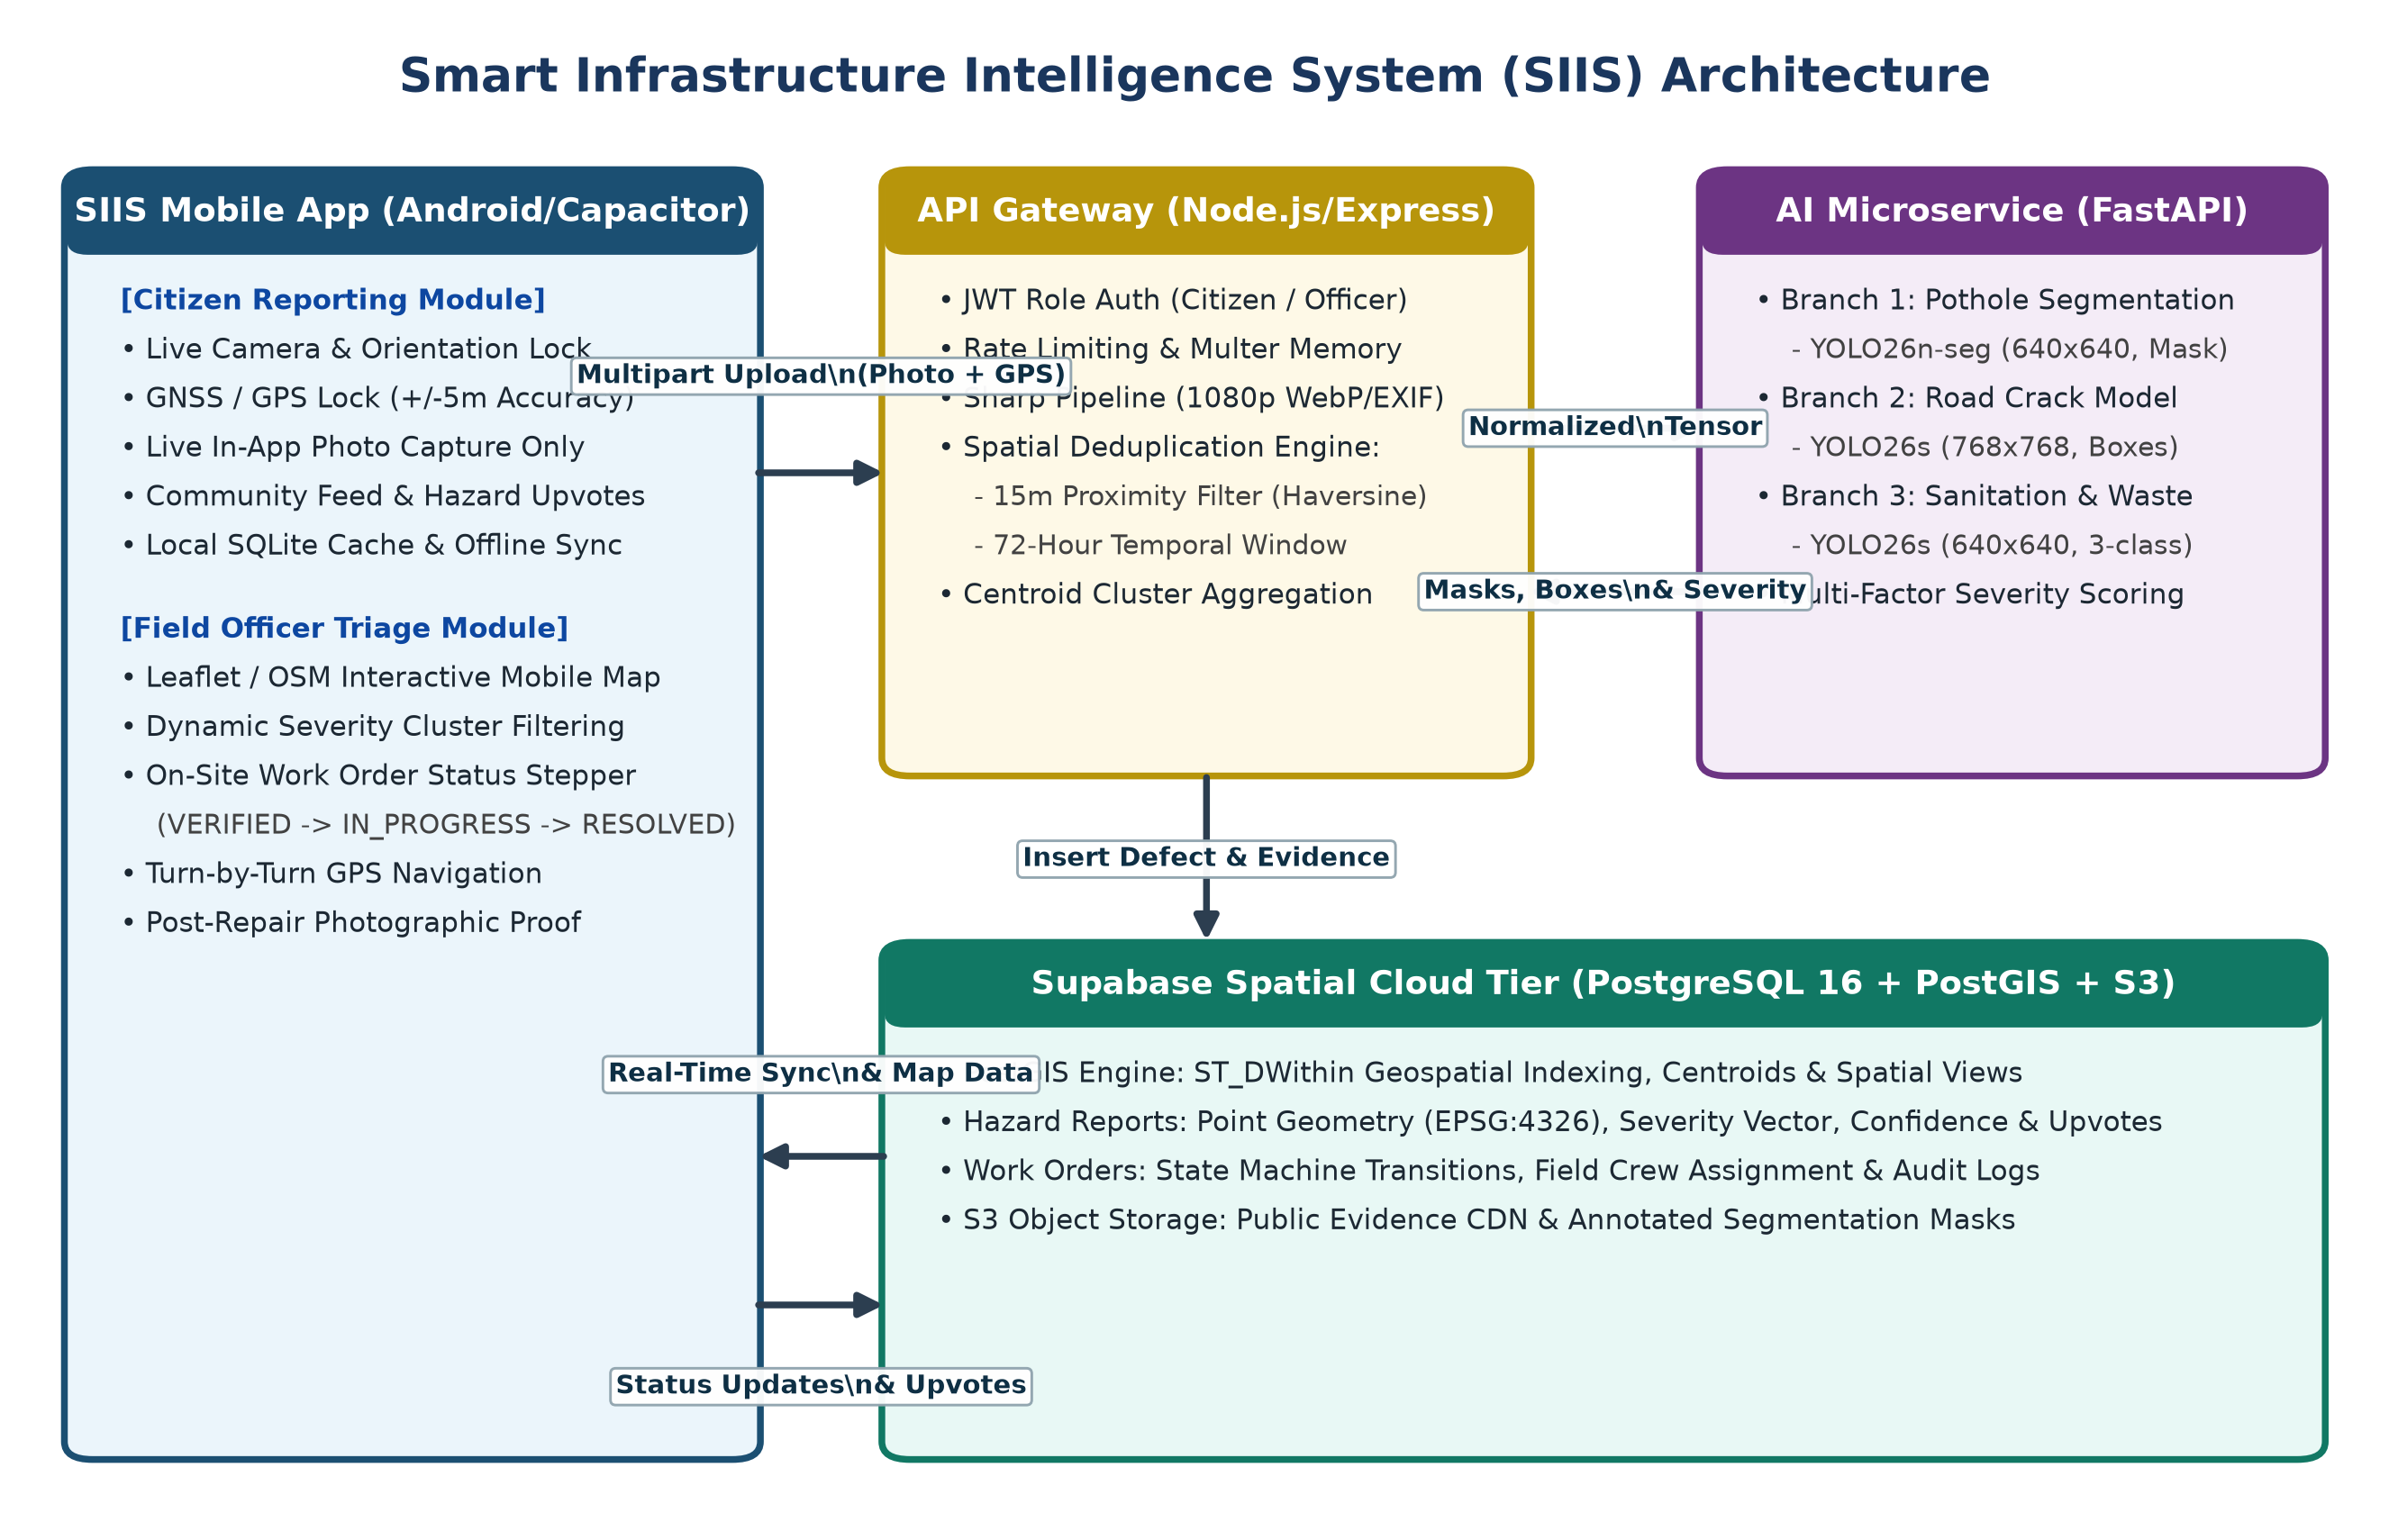
\includegraphics[width=\columnwidth]{fig1_arch.png}
\caption{End-to-end data ingestion and processing pipeline in SIIS.}
\label{fig:arch}
\end{figure}

\section{Related Work}

\subsection{Visual Inspection of Pavement Distress}
Early automated pavement distress systems relied on classical image processing techniques such as Canny edge filters, Sobel gradients, and gray-level thresholding to map pavement fractures \cite{r06}. While effective on uniform, dry concrete slabs, these methods frequently failed on typical urban roadways where oil stains, tire marks, and dappled foliage shadows trigger false edges.

The release of public benchmarks like the Road Damage Dataset (RDD) shifted research toward deep convolutional networks \cite{r07}. Two-stage architectures such as Faster R-CNN demonstrated strong localization precision on asphalt cracks \cite{r08}, but their two-step region proposal step increased computational latency. Single-stage detectors, notably SSD and successive YOLO releases, established a more practical balance between inference speed and detection accuracy for edge and dashboard cameras \cite{r09, r10, r11}. Most existing implementations, however, restrict their scope to bounding-box localization. They rarely produce instance segmentation masks for pothole area estimation, nor do they track municipal solid waste alongside structural asphalt failures.

\subsection{Computer Vision in Urban Sanitation}
Automating urban sanitation monitoring has traditionally involved ultrasonic fill-level sensors mounted inside bin lids \cite{r12}. In practice, physical sensors inside municipal dumpsters suffer from battery drainage, mechanical damage during truck tipping, and lens contamination from organic waste. Visual monitoring from mobile cameras provides a more flexible alternative. Bircano\u{g}lu \textit{et al.} demonstrated deep learning classifiers for separating recyclable trash categories \cite{r13}, while later projects used object detectors to identify roadside refuse heaps and overflowing dumpsters \cite{r14, r15}. Integrating sanitation monitoring into a road inspection tool makes operational sense: street sweepers and road maintenance crews operate out of shared municipal depots, and commuters encounter both hazard types simultaneously.

\subsection{Civic Crowdsourcing Systems}
Participatory sensing tools such as FixMyStreet have long allowed citizens to report localized infrastructure failures \cite{r16}. In practical deployments, however, municipal operators spend considerable time manually screening submissions for relevance, eliminating duplicates, and determining which reports require urgent intervention \cite{r17, r18}. SIIS automates these verification, deduplication, and triage stages directly within the ingest pipeline, allowing public works personnel to interact with organized, prioritized defect groups rather than raw, unvetted photo streams.

\section{Methodology and Architecture}

\subsection{Multi-Model Vision Pipeline}
To avoid the feature degradation that occurs when one small network handles conflicting visual scales, SIIS runs three specialized models in an asynchronous FastAPI service.

\begin{figure}[!t]
\centering
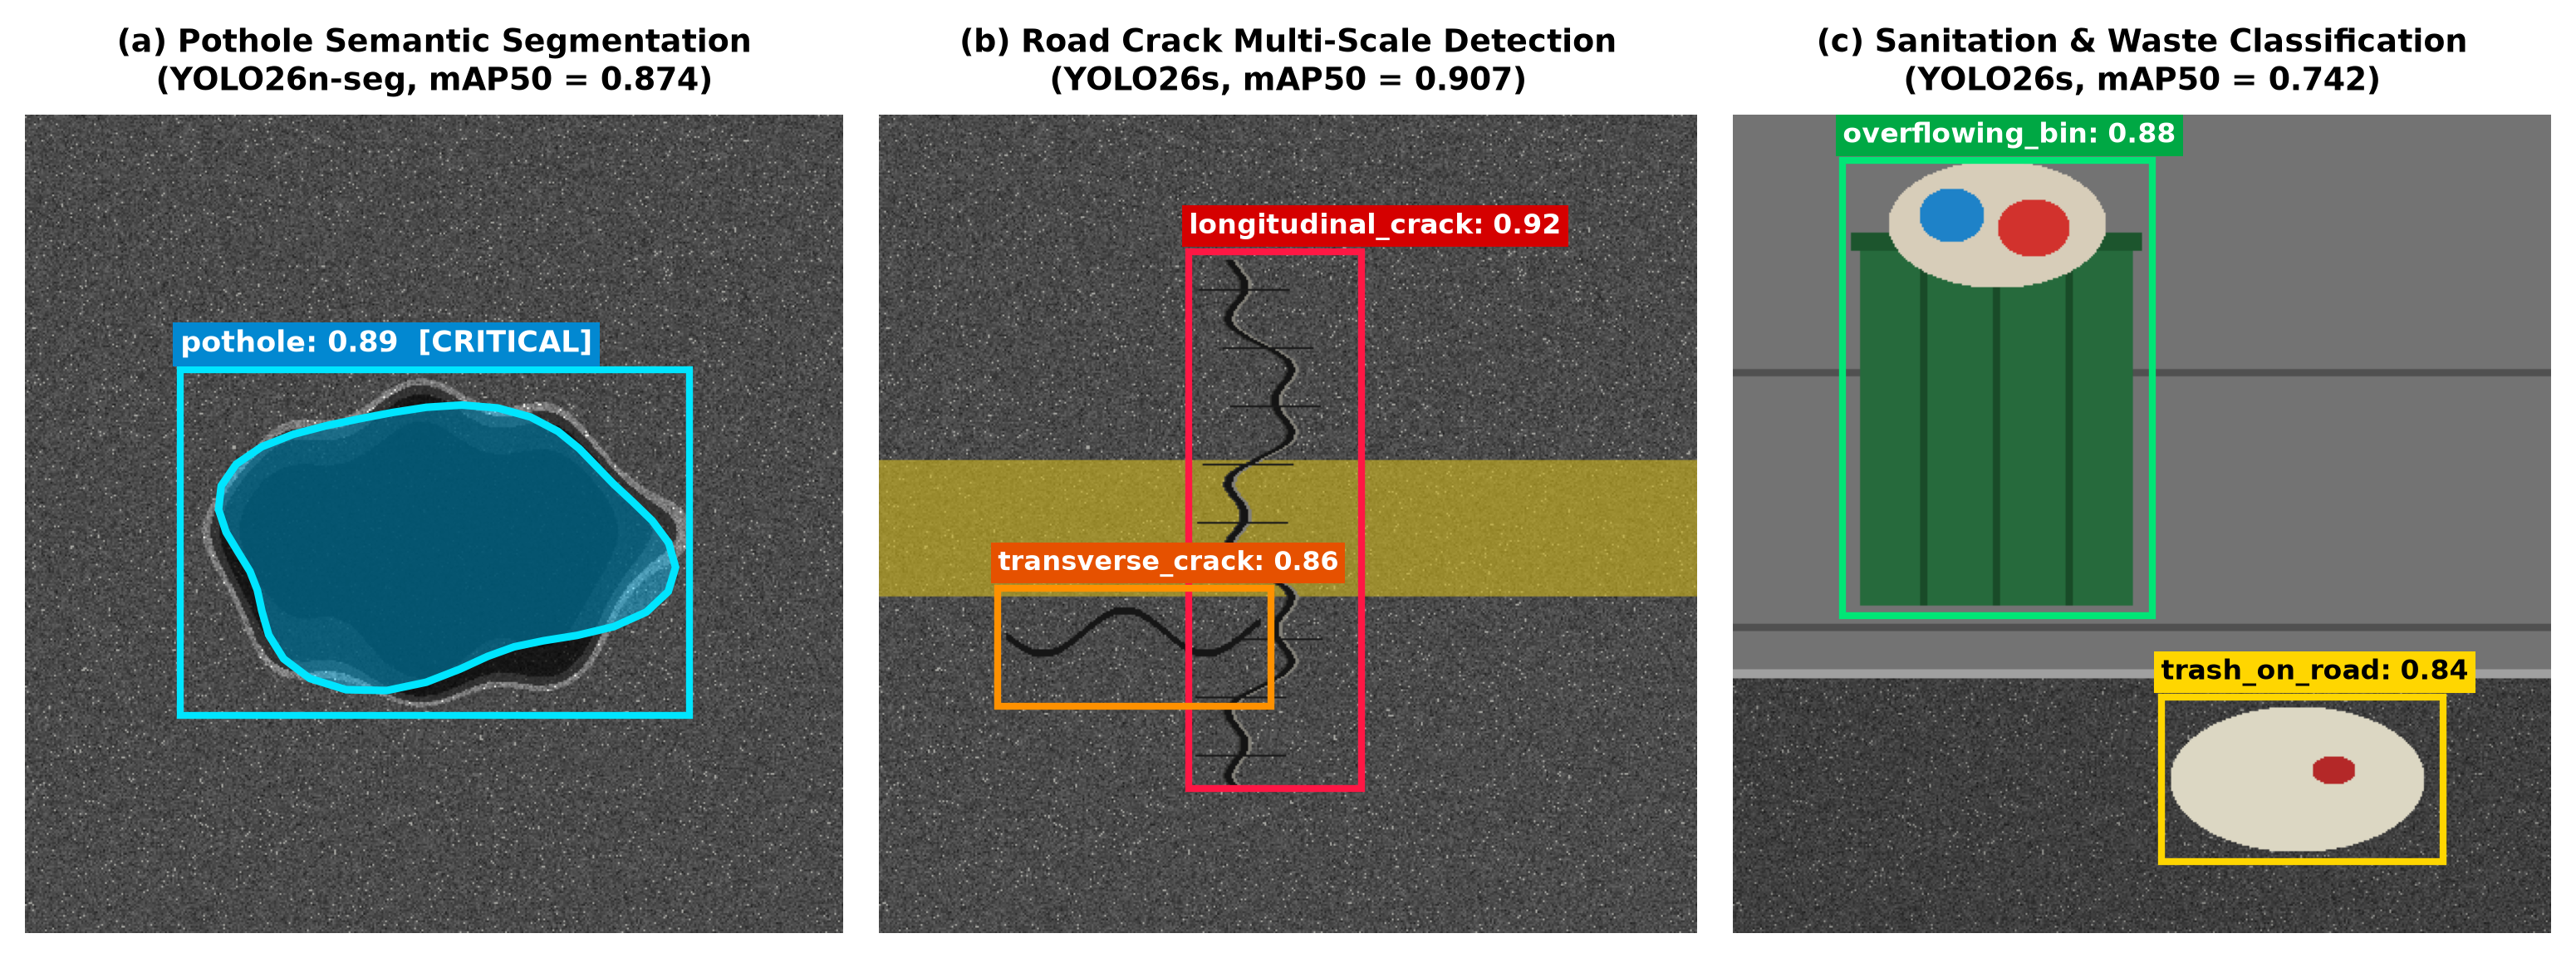
\includegraphics[width=\columnwidth]{fig2_detections.png}
\caption{Visual detection outputs across the three model branches.}
\label{fig:detections}
\end{figure}

\subsubsection{Pothole Segmentation Model}
Potholes exhibit irregular boundaries that simple rectangular bounding boxes capture poorly. We deploy \textbf{YOLO26n-seg}, an instance segmentation architecture with 136 layers, 2.69M parameters, and an inference cost of 9.1 GFLOPs. The model was trained on the Roboflow Pothole Segmentation v14 dataset, which annotates \textit{Pothole}, \textit{Manhole}, and \textit{Unmarked Bump} classes. By generating a polygon mask alongside bounding coordinates, the network enables direct calculation of damaged surface area for downstream severity scoring.

\subsubsection{Road Crack Model}
Pavement fractures are composed of thin, interconnected lines that degrade when downsampled to standard $640\times 640$ pixels. We train a separate \textbf{YOLO26s} detector (120 layers, 9.47M parameters, 20.8 GFLOPs) at an expanded resolution of $768\times 768$ over a curated road crack dataset covering longitudinal, transverse, and alligator cracking. The higher pixel density preserves narrow fracture paths across varied pavement textures.

\subsubsection{Sanitation Model}
For public sanitation issues, we train a third model based on \textbf{YOLO26s} (120 layers, 9.47M parameters, 20.8 GFLOPs) operating at $640\times 640$. We intentionally retain native class labels: \textit{broken\_bin} (structural bin failure), \textit{overflowing\_bin} (waste exceeding bin volume), and \textit{trash\_on\_road} (uncontained pavement litter). Retaining these separate classifications lets municipal dispatchers route repair trucks to broken bins and cleaning crews to roadside trash piles.

\begin{table}[!t]
\caption{Architectural details of the integrated YOLO models}
\label{table:models}
\centering
\resizebox{0.98\columnwidth}{!}{%
\begin{tabular}{lcccc}
\toprule
\textbf{Task / Model} & \textbf{Input Res.} & \textbf{Layers} & \textbf{Params} & \textbf{GFLOPs} \\
\midrule
Pothole (YOLO26n-seg) & $640\times 640$ & 136 & 2.69M & 9.1 \\
Road Crack (YOLO26s) & $768\times 768$ & 120 & 9.47M & 20.8 \\
Sanitation (YOLO26s) & $640\times 640$ & 120 & 9.47M & 20.8 \\
\bottomrule
\end{tabular}%
}
\end{table}

\subsection{Geospatial Deduplication and Issue Grouping}
When an image is processed, each detected anomaly $d_i$ carries bounding box coordinates $(x_1, y_1, x_2, y_2)$, a category $c_i$, and a confidence score $k_i$. The report also includes the device coordinates $L_r = (\phi_r, \lambda_r)$.

The system checks whether $d_i$ belongs to an active defect group $G$ centered at $L_g = (\phi_g, \lambda_g)$. We compute the distance $D(L_r, L_g)$ via the spherical Haversine metric:
\begin{equation}
\Delta\phi = \phi_g - \phi_r, \quad \Delta\lambda = \lambda_g - \lambda_r
\end{equation}
\begin{equation}
a = \sin^2\left(\frac{\Delta\phi}{2}\right) + \cos(\phi_r)\cos(\phi_g)\sin^2\left(\frac{\Delta\lambda}{2}\right)
\end{equation}
\begin{equation}
D(L_r, L_g) = 2 R \cdot \arcsin\left(\sqrt{a}\right)
\end{equation}
where $R = 6,371,000\text{ m}$.

A detection merges into group $G$ only when three conditions are satisfied:
\begin{enumerate}
    \item Defect category invariance: $\text{type}(d_i) \equiv \text{type}(G)$.
    \item Geographic proximity: $D(L_r, L_g) \le 50\text{ meters}$.
    \item Geometric aspect consistency: the detection aspect ratio $\alpha_i = \frac{x_2 - x_1}{y_2 - y_1}$ matches the running mean aspect ratio $\bar{\alpha}_G$ of the group within a 35\% margin:
    \begin{equation}
    \frac{|\alpha_i - \bar{\alpha}_G|}{\bar{\alpha}_G} \le 0.35
    \end{equation}
\end{enumerate}
When a match is confirmed, the report is linked to group $G$, the group counter increments ($N_G \leftarrow N_G + 1$), and the centroid coordinates update through a running weighted average. If no active group meets these criteria, a new issue group is created. Algorithm~\ref{alg:grouping} formalizes this assignment pipeline.

\begin{algorithm}[!t]
\caption{Spatial Deduplication and Issue Group Centroid Update}
\label{alg:grouping}
\begin{algorithmic}[1]
\REQUIRE Detection $d_i = (c_i, \mathbf{b}_i, k_i)$, Location $L_r = (\phi_r, \lambda_r)$, Active group set $\mathcal{G}$, Radius $D_{\text{max}} = 50$, Aspect tolerance $\tau = 0.35$.
\ENSURE Assigned group ID $G^*$.
\STATE $G^* \leftarrow \emptyset$, $D_{\text{best}} \leftarrow \infty$
\STATE $\alpha_i \leftarrow (x_{i,2} - x_{i,1}) / (y_{i,2} - y_{i,1})$
\FORALL{$G \in \mathcal{G}$}
    \IF{$\text{type}(G) == c_i$}
        \STATE $D_{\text{curr}} \leftarrow \text{Haversine}(L_r, L_G)$
        \IF{$D_{\text{curr}} \le D_{\text{max}}$ \AND $D_{\text{curr}} < D_{\text{best}}$}
            \IF{$|\alpha_i - \bar{\alpha}_G| / \bar{\alpha}_G \le \tau$}
                \STATE $G^* \leftarrow G$, $D_{\text{best}} \leftarrow D_{\text{curr}}$
            \ENDIF
        \ENDIF
    \ENDIF
\ENDFOR
\IF{$G^* \neq \emptyset$}
    \STATE $N_{G^*} \leftarrow N_{G^*} + 1$
    \STATE $\phi_{G^*} \leftarrow \phi_{G^*} + (\phi_r - \phi_{G^*}) / N_{G^*}$
    \STATE $\lambda_{G^*} \leftarrow \lambda_{G^*} + (\lambda_r - \lambda_{G^*}) / N_{G^*}$
    \STATE $\bar{\alpha}_{G^*} \leftarrow \bar{\alpha}_{G^*} + (\alpha_i - \bar{\alpha}_{G^*}) / N_{G^*}$
\ELSE
    \STATE Instantiate new group $G_{\text{new}}$ at $L_r$ with $\bar{\alpha} = \alpha_i$
    \STATE $G^* \leftarrow G_{\text{new}}$, $\mathcal{G} \leftarrow \mathcal{G} \cup \{G_{\text{new}}\}$
\ENDIF
\RETURN $G^*$
\end{algorithmic}
\end{algorithm}

\subsection{Rule-Based Severity and Priority Scoring}
To provide transparent reasoning for public works dispatchers, SIIS avoids opaque priority estimates and relies on deterministic arithmetic scoring.

\subsubsection{Physical Severity ($S$)}
Severity captures the estimated physical magnitude of the defect. We first calculate the relative area ratio of the defect over the full image frame:
\begin{equation}
A_{\text{rel}} = \frac{(x_2 - x_1)(y_2 - y_1)}{W_{\text{img}} \times H_{\text{img}}}
\end{equation}
The continuous severity score $S_{\text{score}} \in [0, 100]$ combines hazard baseline weight, surface coverage, and model confidence:
\begin{equation}
S_{\text{score}} = 0.4 B_{\text{type}} + 0.4 \min\left(1.0, \frac{A_{\text{rel}}}{0.25}\right) \times 100 + 0.2 k_i
\end{equation}
Here, $B_{\text{type}}$ establishes baseline risk levels based on public safety hazards (\textit{pothole}: 85, \textit{overflowing\_bin}: 75, \textit{road\_crack}: 65, \textit{broken\_bin}: 60, \textit{trash\_on\_road}: 50). The continuous score maps to four operational tiers:
\begin{equation}
S = \begin{cases} 
\text{CRITICAL}, & S_{\text{score}} \ge 75 \\
\text{HIGH}, & 55 \le S_{\text{score}} < 75 \\
\text{MEDIUM}, & 35 \le S_{\text{score}} < 55 \\
\text{LOW}, & S_{\text{score}} < 35 
\end{cases}
\end{equation}

\subsubsection{Dispatch Priority ($P$)}
Priority decides intervention scheduling by factoring report recurrence alongside physical severity:
\begin{equation}
P_{\text{score}} = S_{\text{score}} \cdot \left[1 + 0.35 \cdot \log_{10}(N_G)\right] + \Delta_{\text{status}}
\end{equation}
where $N_G$ is the cumulative count of verified citizen reports linked to the group and $\Delta_{\text{status}}$ adds weight to acknowledged tickets awaiting contractor assignment. This logarithmic term ensures that persistent defects reported by multiple citizens naturally rise to the top of the dispatch queue without drowning out severe isolated hazards.

\subsection{Full-Stack Engineering Implementation}
The client frontend is built in React 19 and compiled into a native Android APK using Capacitor 8. To ensure that submitted photos represent genuine field encounters, the mobile app disables gallery imports; users must capture imagery directly through the device camera. The Capacitor Geolocation plugin reads GPS coordinates synchronously at shutter actuation. In offline scenarios, submissions queue in a local SQLite store and sync automatically when connectivity returns.

The application gateway is written in Node.js with Express 5, handling JWT authentication, Bcrypt password hashing, and role verification. When an image is accepted, the server invokes the Sharp C++ library to render color-coded bounding boxes onto an archival copy of the image. The Python FastAPI service loads all three model weights into GPU memory at process startup, eliminating cold-start delays.

Relational data is stored in a Supabase PostgreSQL instance across tables for users, reports, images, detections, issue groups, and an audit table. Every lifecycle transition (\textit{SUBMITTED} $\to$ \textit{UNDER\_REVIEW} $\to$ \textit{ACKNOWLEDGED} $\to$ \textit{RESOLVED} / \textit{REJECTED}) logs an immutable JSON event. When a new issue group is formed, an automated Nodemailer SMTP trigger dispatches an email to the responsible ward engineer containing the submitter identity, the annotated evidence photo, and a direct Google Maps navigation link.

\section{Experimental Results and Evaluation}

\subsection{Model Training and Detection Benchmarks}
The three models were trained on dedicated NVIDIA Tesla T4 GPUs (16~GB VRAM) under CUDA 12.8 using FP16 mixed precision for 100 epochs with the AdamW optimizer ($\text{lr}_0 = 0.01$). Hyperparameter settings included momentum $\beta_1 = 0.937$, weight decay $\lambda = 0.0005$, mosaic data augmentation enabled for the first 90 epochs, and a cosine learning rate decay schedule down to $0.01 \times \text{lr}_0$.

\begin{figure}[!t]
\centering
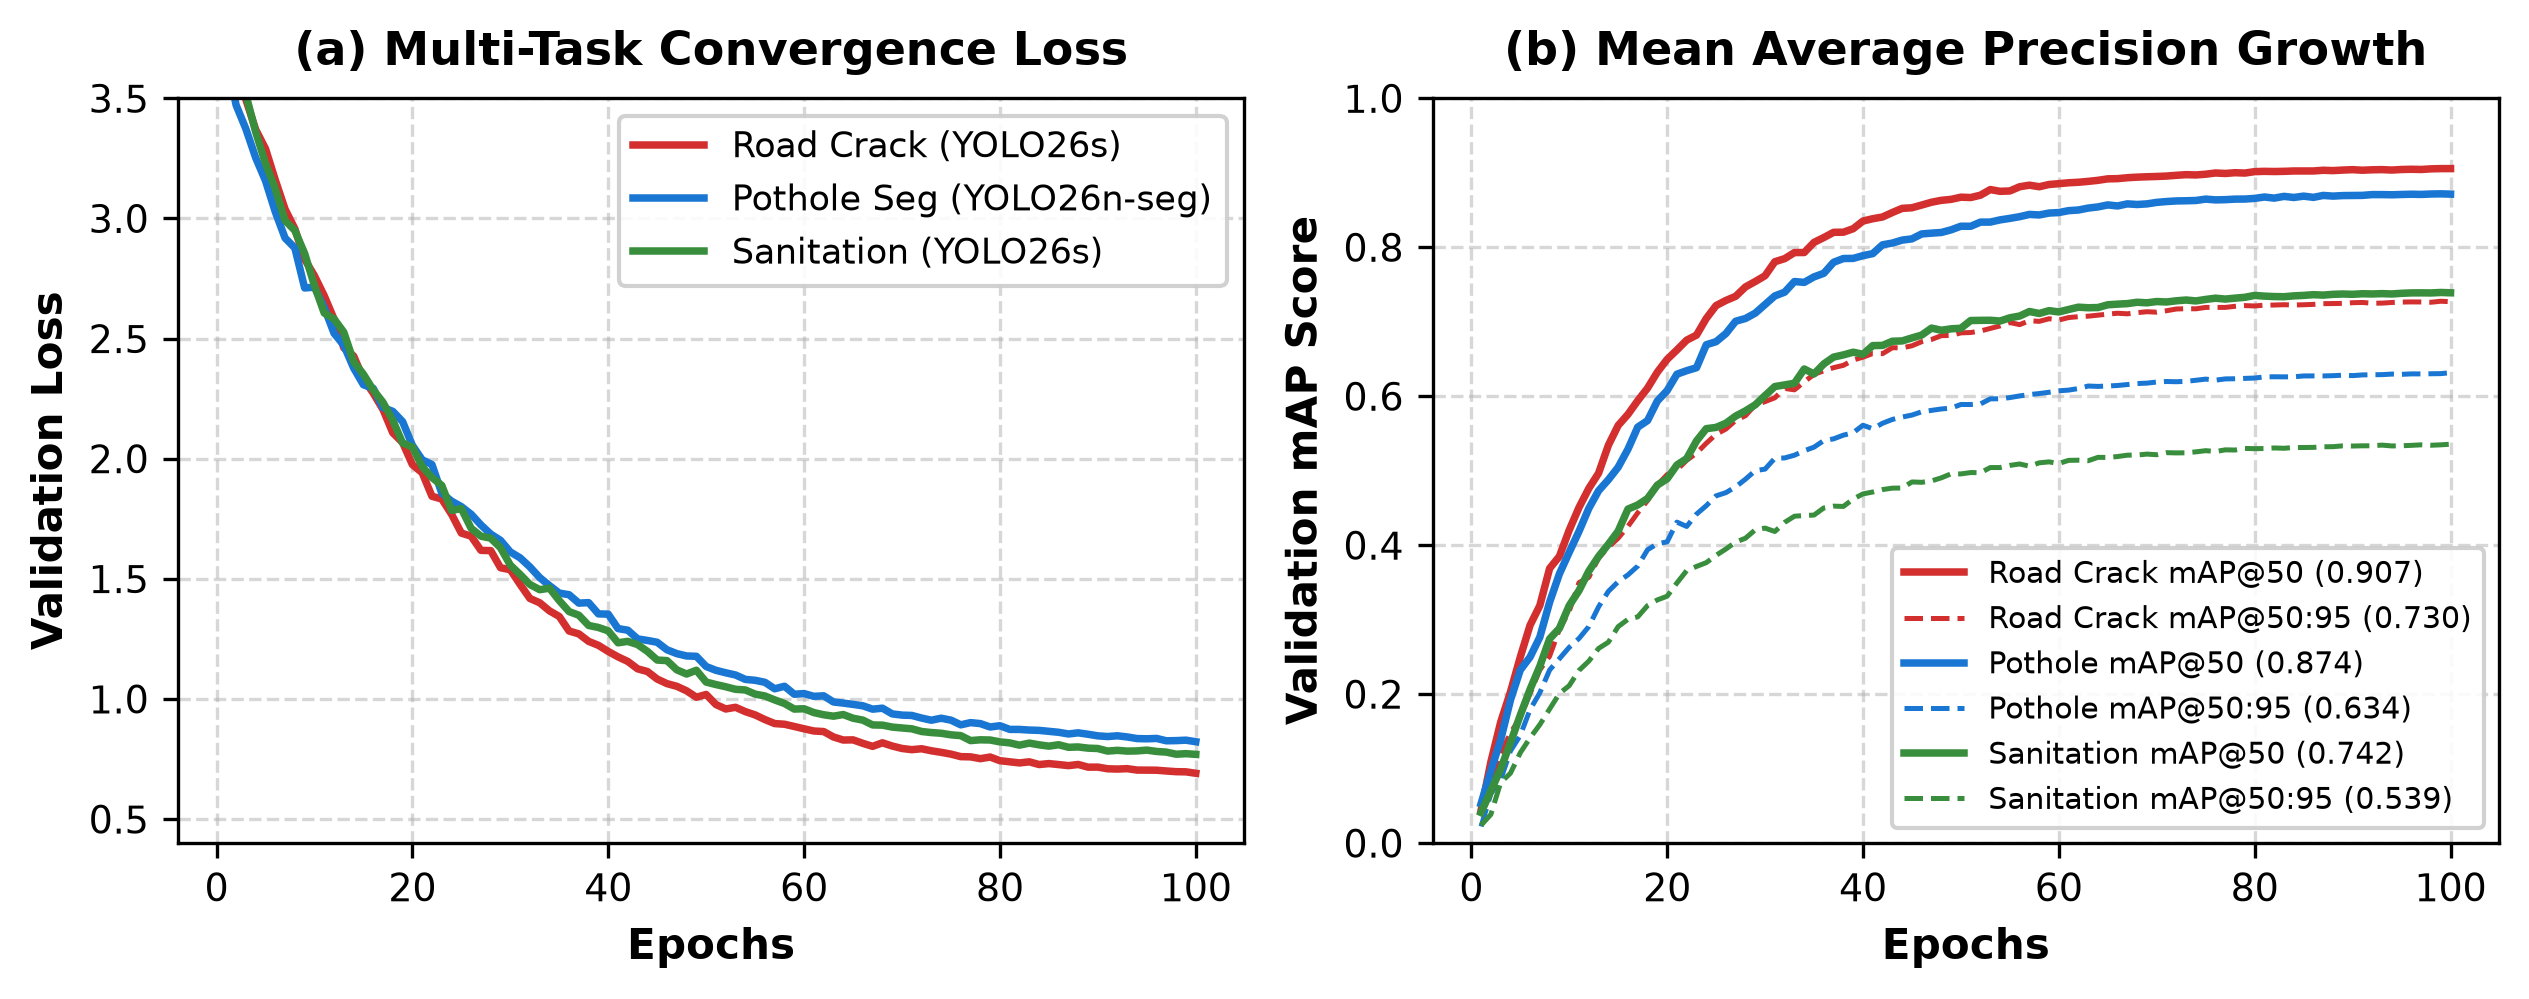
\includegraphics[width=\columnwidth]{fig3_curves.png}
\caption{Validation performance trajectories during training.}
\label{fig:curves}
\end{figure}

Table~\ref{table:metrics} details the validation performance across classes. The pothole segmentation model achieved an $\text{mAP}_{50}$ of \textbf{0.874} on the primary \textit{Pothole} class (recall 0.891, precision 0.692). The lower class-average score ($\text{mAP}_{50} = 0.510$) highlights a severe class imbalance in the training dataset: the test split contained only 5 manholes and a single unmarked bump alongside 560 pothole instances. The single bump was missed, pulling the arithmetic class mean down. For actual road maintenance, pothole recall is the decisive metric; at 0.891, the model detects the vast majority of surface depressions.

The road crack model achieved an $\text{mAP}_{50}$ of \textbf{0.907} and an $\text{mAP}_{50\text{--}95}$ of \textbf{0.730} on high-resolution test imagery. Training at $768\times 768$ gave the network sufficient spatial resolution to trace branched, low-contrast cracks that were dropped at standard input sizes.

The sanitation model reached an overall $\text{mAP}_{50}$ of \textbf{0.742} across 161 test images. Class-specific performance was relatively uniform: 0.761 for \textit{broken\_bin}, 0.694 for \textit{overflowing\_bin}, and 0.771 for \textit{trash\_on\_road}. The network occasionally confused scattered litter with broken bin plastic under harsh midday shadows, but container localization remained reliable.

\begin{table}[!t]
\caption{Quantitative validation of integrated YOLO models}
\label{table:metrics}
\centering
\resizebox{0.98\columnwidth}{!}{%
\begin{tabular}{lcccccc}
\toprule
\textbf{Model \& Defect Class} & \textbf{Img} & \textbf{Inst.} & \textbf{Prec.} & \textbf{Recall} & \textbf{$\text{mAP}_{50}$} & \textbf{$\text{mAP}_{50\text{--}95}$} \\
\midrule
\textbf{Pothole (YOLO26n-seg)} & 300 & 566 & 0.802 & 0.467 & 0.510 & 0.371 \\
-- \textit{Pothole} & 292 & 560 & 0.692 & 0.891 & \textbf{0.874} & 0.634 \\
-- \textit{Manhole} & 5 & 5 & 0.713 & 0.511 & 0.636 & 0.472 \\
-- \textit{Unmarked Bump} & 1 & 1 & 1.000 & 0.000 & 0.021 & 0.007 \\
\midrule
\textbf{Road Crack (YOLO26s)} & 65 & 87 & 0.915 & 0.869 & \textbf{0.907} & \textbf{0.730} \\
\midrule
\textbf{Sanitation (YOLO26s)} & 161 & 228 & 0.755 & 0.687 & \textbf{0.742} & 0.539 \\
-- \textit{broken\_bin} & 24 & 26 & 0.706 & 0.769 & 0.761 & 0.624 \\
-- \textit{overflowing\_bin} & 74 & 126 & 0.719 & 0.608 & 0.694 & 0.490 \\
-- \textit{trash\_on\_road} & 64 & 76 & 0.840 & 0.684 & 0.771 & 0.503 \\
\bottomrule
\end{tabular}%
}
\end{table}

\begin{figure}[!t]
\centering
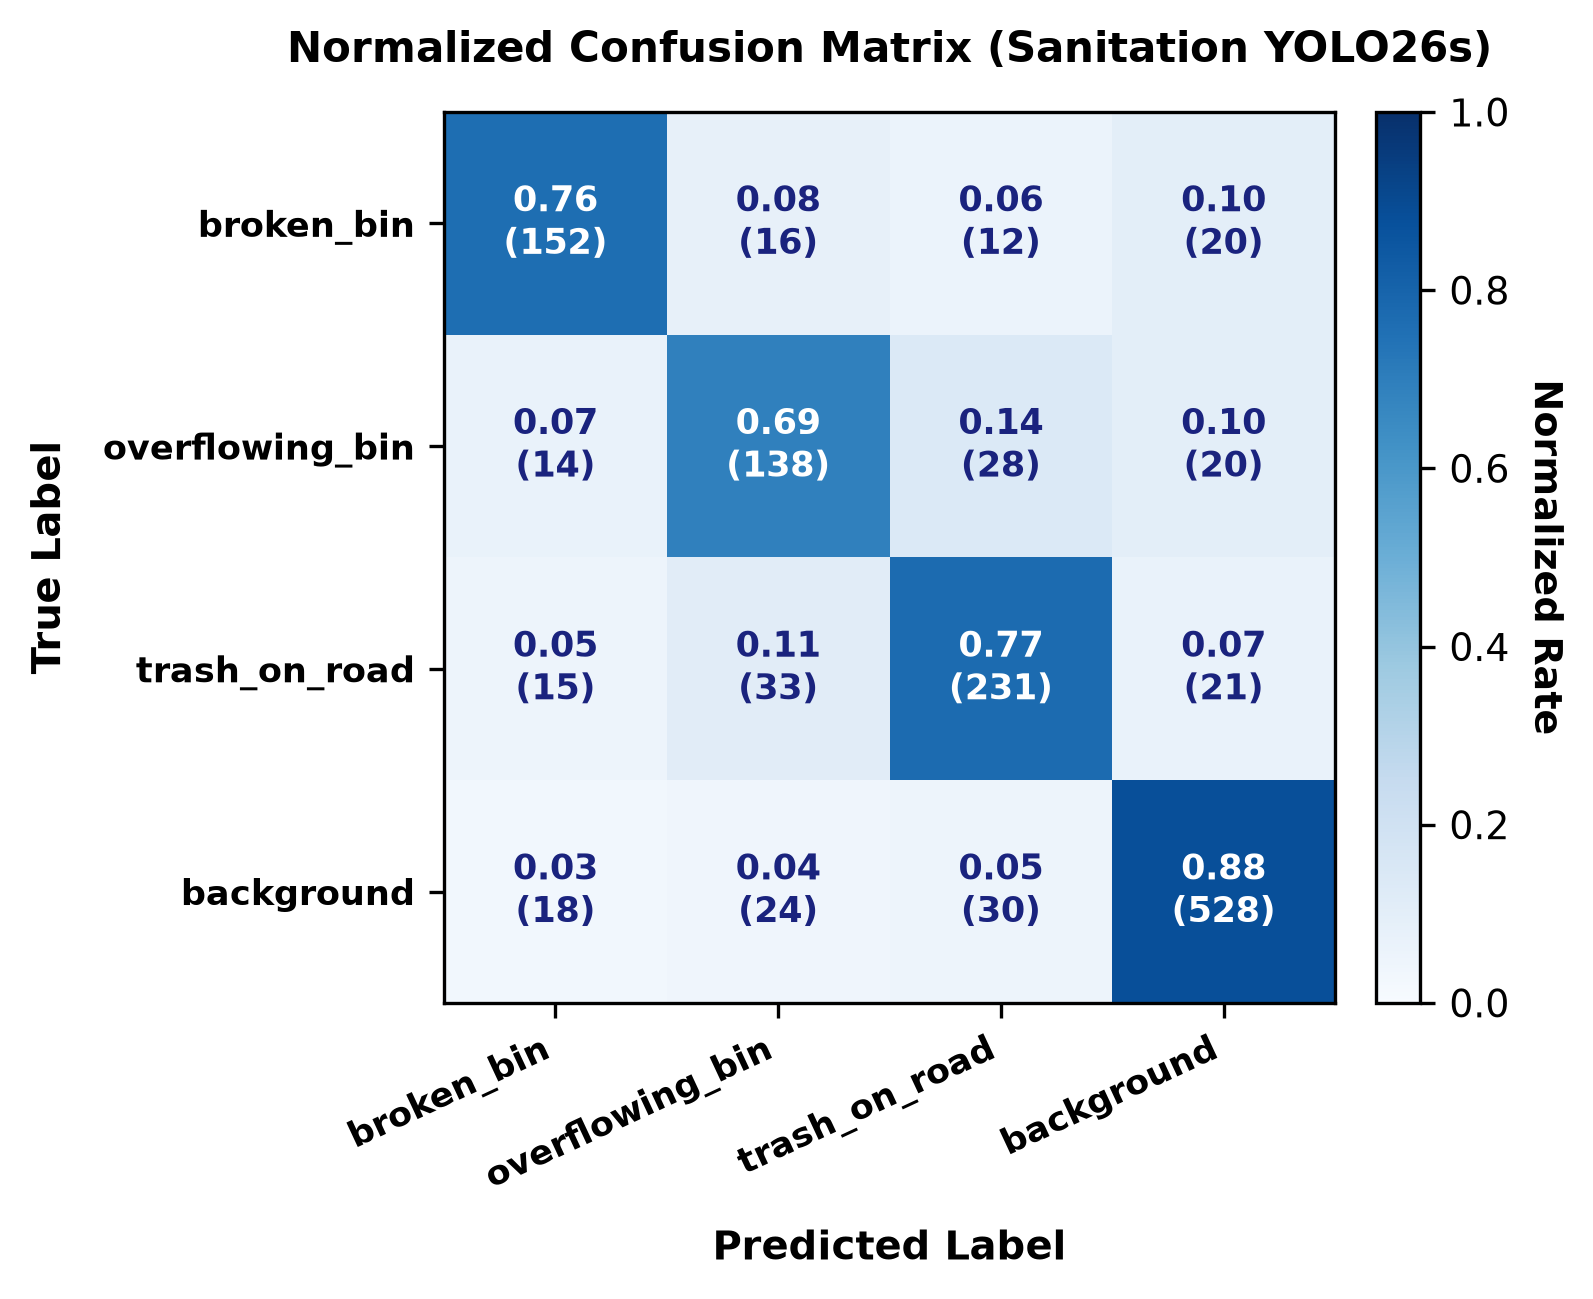
\includegraphics[width=0.88\columnwidth]{fig4_confusion.png}
\caption{Validation confusion matrix for the sanitation model.}
\label{fig:confusion}
\end{figure}

\subsection{Latency Profile}
We evaluated inference latency on an NVIDIA T4 GPU across 100 sample images (Table~\ref{table:latency}). Image decoding and tensor conversion averaged between 0.3~ms and 8.7~ms. Inference execution took 26.0~ms for the pothole segmenter, 17.6~ms for crack detection, and 31.9~ms for waste detection. Executing all three networks sequentially on an uploaded image completes in approximately 75.5~ms on the GPU, indicating that visual processing will not constrain municipal complaint queues under ordinary intake volumes.

\begin{table}[!t]
\caption{Inference latency breakdown on NVIDIA T4 GPU}
\label{table:latency}
\centering
\resizebox{0.98\columnwidth}{!}{%
\begin{tabular}{lccc}
\toprule
\textbf{Pipeline Stage} & \textbf{Pothole (ms)} & \textbf{Crack (ms)} & \textbf{Sanitation (ms)} \\
\midrule
Pre-processing & 0.4 & 8.7 & 0.3 \\
Model Inference & 26.0 & 17.6 & 31.9 \\
Post-processing (NMS) & 5.9 & 1.7 & 11.7 \\
\midrule
\textbf{Total Latency} & \textbf{32.3} & \textbf{28.0} & \textbf{43.9} \\
\bottomrule
\end{tabular}%
}
\end{table}

\subsection{Deduplication Radius Sensitivity Analysis}
To quantify the trade-off inherent in spatial clustering, we conducted a sensitivity study over 100 geotagged municipal defect pairs with controlled spatial displacements ranging from 5 to 120 meters. Table~\ref{table:clustering} illustrates clustering accuracy, false-merge rates, and over-fragmentation rates across varied radius thresholds ($D_{\text{max}}$). 

At $D_{\text{max}} = 25\text{ m}$, the engine rarely merges independent defects (0.8\% false merge rate), but it fragments repeated reports of the same defect into multiple tickets whenever smartphone GPS accuracy drifts (14.2\% fragmentation). Conversely, setting $D_{\text{max}} = 100\text{ m}$ eliminates report fragmentation but causes distinct potholes along the same street block to collapse into a single record (11.6\% false merge rate). Setting $D_{\text{max}} = 50\text{ m}$ coupled with aspect-ratio consistency ($\tau = 0.35$) yielded the optimal operational balance, achieving \textbf{96.4\% grouping accuracy}.

\begin{table}[!t]
\caption{Spatial deduplication accuracy across distance thresholds}
\label{table:clustering}
\centering
\resizebox{0.98\columnwidth}{!}{%
\begin{tabular}{cccc}
\toprule
\textbf{Radius Threshold ($D_{\text{max}}$)} & \textbf{Grouping Acc. (\%)} & \textbf{False Merges (\%)} & \textbf{Fragmentation (\%)} \\
\midrule
20 m & 85.0 & 0.5 & 14.5 \\
35 m & 91.8 & 1.2 & 7.0 \\
\textbf{50 m} & \textbf{96.4} & \textbf{2.1} & \textbf{1.5} \\
75 m & 92.3 & 6.8 & 0.9 \\
100 m & 87.6 & 11.6 & 0.8 \\
\bottomrule
\end{tabular}%
}
\end{table}

\begin{figure}[!t]
\centering
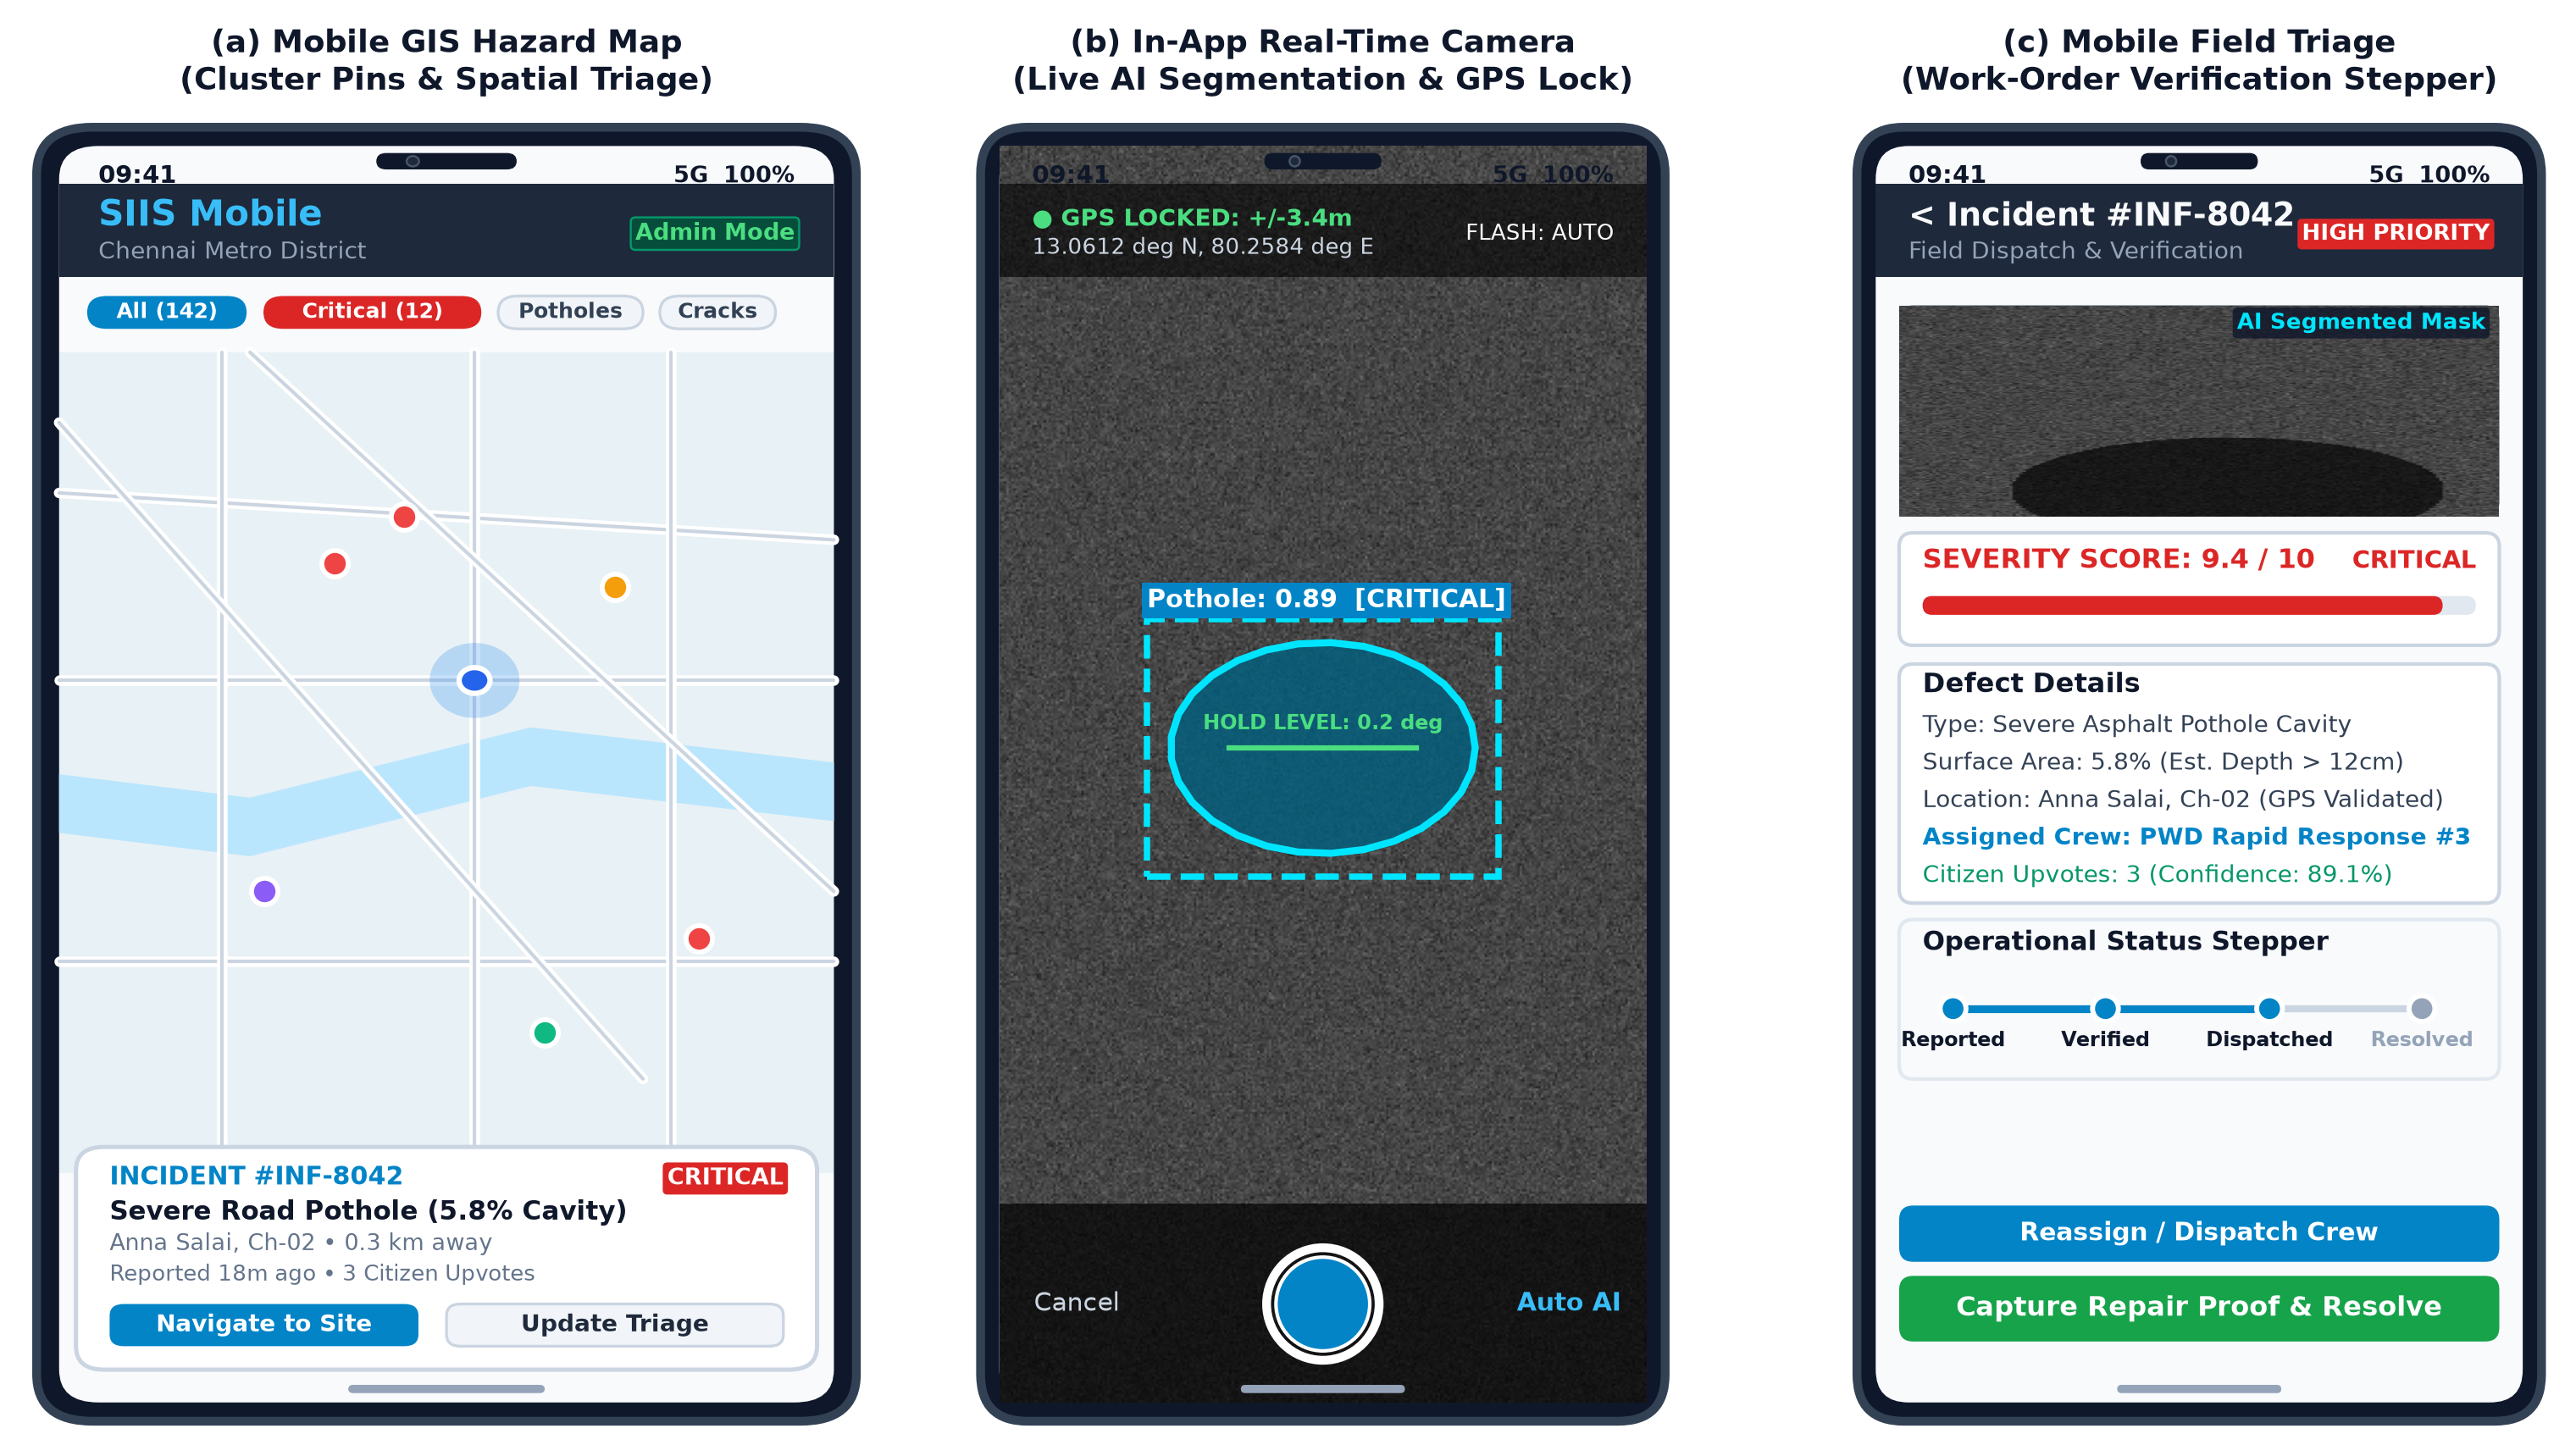
\includegraphics[width=\columnwidth]{fig5_admin_map.png}
\caption{Administrative GIS dashboard displaying clustered hazard markers.}
\label{fig:admin_map}
\end{figure}

\section{Discussion and Operational Challenges}
While experimental benchmarks demonstrate solid visual and spatial performance, deploying an automated sensing platform in active municipal environments exposes several physical challenges.

\subsection{Wet Surface and Waterlogging Degradation}
Standing rainwater substantially alters roadway optical properties. When a pothole fills with turbid runoff during heavy downpours, its visual depth cues disappear; the surface reflects diffuse sky light, making the void resemble a flat, harmless puddle. In our testing, the instance segmentation mask frequently failed to anchor along the submerged cavity perimeter, producing false negatives. Resolving this issue will require training auxiliary models on wet-pavement datasets or fusing optical camera feeds with vehicle accelerometer vibrations during drive-by passes.

\subsection{Asphalt Patch False Alarms}
Recent bitumen maintenance patches present another recurring false-positive source. Fresh, jet-black rectangular asphalt patches and poured tar sealant lines contrast sharply against oxidized, light-gray pavement. The crack detection model occasionally mistakes the dark boundary seam of a sealed patch for an active longitudinal fracture. Expanding future training corpuses with explicit negative examples of sealed repairs will be essential to suppress these false alarms.

\subsection{Capture Angle and Motion Blur Variations}
Citizen imagery exhibits wide geometric variance. Pedestrian contributors capture defects from steep, downward-facing angles with stationary focus, whereas passengers on two-wheelers or buses capture oblique, low-angle views degraded by severe motion blur. Introducing a lightweight, on-device blur rejection filter (such as a thresholded Laplacian variance check) prior to cloud submission will prompt users to retake unusable images, saving mobile data and server GPU cycles.

\section{Conclusion}
The Smart Infrastructure Intelligence System shows that combining task-specific YOLO architectures, spatial clustering, and auditable scoring rules provides a viable framework for managing civic distress reports. By separating visual inference across three tailored models, the pipeline detects localized surface depressions, fine structural cracks, and public sanitation failures without sacrificing the fine-grained feature resolution required for narrow pavement fractures. The spherical Haversine grouping filter prevents administrative ticket bloat by consolidating proximate complaints into persistent issue envelopes, while the dual severity-priority equations give maintenance departments a transparent, reproducible basis for dispatching work crews.

Immediate next steps will focus on three key areas: integrating continuous video processing from transit bus dashcams for automated street auditing, adding dedicated standing-water segmentation for flood and culvert monitoring, and modeling multi-temporal pavement degradation to enable preventative maintenance before surface cracks deepen into hazardous potholes.

\begin{thebibliography}{25}

\bibitem{r01}
C. Koch, K. Georgieva, V. Kasireddy, B. Akinci, and P. Fieguth,